\thispagestyle{fancy}

\begin{center}
  {\LARGE\bfseries Message from the Principal\par}
\end{center}

\vspace{0.7cm}
\noindent
\begin{minipage}[c]{0.22\textwidth}
  \centering
  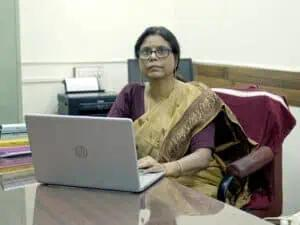
\includegraphics[width=\linewidth]{assets/images/principal_shila_ghosh.jpg}
\end{minipage}
\hfill
\begin{minipage}[c]{0.73\textwidth}
  {\large\bfseries Prof. (Dr.) Shila Ghosh\par}
  \smallskip
  {\itshape Professor \& Principal\par}
\end{minipage}

\vspace{0.7cm}
{\justifying
It gives me immense pleasure to share a few words on the publication of Volume X of \textit{Electronic Trends}, the Departmental Technical Magazine of Electronics \& Communication Engineering. This magazine reflects the curiosity, creativity, and enthusiasm of our students and faculty members, while also highlighting the department's continued commitment to technical excellence, research, innovation, and all-round development.

\medskip
Every edition provides an opportunity to celebrate the ideas, achievements, and collaborative efforts that strengthen our academic community. Volume X carries this tradition forward through thoughtful technical articles, emerging-technology discussions, student contributions, project insights, and glimpses of the academic and co-curricular activities undertaken during the year.

\medskip
I sincerely appreciate the editorial board, faculty coordinators, contributors, and student volunteers whose dedication has shaped this edition. Bringing together a publication of this nature requires patience, teamwork, and careful attention to detail. Their efforts have made the magazine both informative and engaging and reflect the values of responsibility and continuous improvement upheld by our institution.

\medskip
I encourage our students to use this platform to express original ideas, share their learning, and develop the confidence to explore beyond the classroom. In a rapidly changing technological world, the willingness to question, experiment, collaborate, and continue learning is as important as technical knowledge itself. I hope this volume inspires its readers to pursue meaningful innovation and approach future challenges with integrity and purpose.

\medskip
I extend my warm congratulations to everyone associated with Volume X and wish the Department of Electronics \& Communication Engineering continued progress and success in all its future endeavours.\par}

\medskip
\begin{flushright}
  \textbf{Prof. (Dr.) Shila Ghosh}\par
  Principal\par
  {\small St. Thomas' College of Engineering \& Technology, Kolkata\par}
\end{flushright}

\vfill\null